\section{Static Multiple-Issue Processor: Approccio VLIM }\label{capitolo4}
Fino ad ora abbiamo analizzato tecniche che permettono di estrapolare il parallelismo dalle istruzioni solo nel caso in cui queste siano prelevate dalla memoria in modo sequenziale una alla volta; con questo meccanismo abbiamo che il CPI massimo che possiamo ottenere è 1 ovvero possiamo eseguire, nel migliore dei casi, al massimo una istruzione per ciclo.\\
Introduciamo ora una categoria di processori che, invece, sono in grado di prelevare più di una istruzione per ogni ciclo di clock. Questi processori possono essere a \emph{scheduler dinamico} ovvero possono prelevare un numero diverso di istruzioni ad ogni ciclo di clock, oppure a scheduler statico che preleva un numero prefissato di istruzioni ad ogni ciclo.\\
Il numero di istruzioni che si possono prelevare ad ogni ciclo può variare da un minimo di 1 ad un massimo di 8 il CPI in questo caso diventa $CPI= 1/ \#istruzioni \ prelevate$. Questo tipo di processore viene definito \emph{processore superscalare}. Lo scheduler può essere implementato esclusivamente tramite lo hardware anche se il compilatore può migliorare notevolmente la qualità dello scheduler. Lo hardware risistema le istruzioni in esecuzione per ridurre il numero degli stalli mentre mantiene il flusso dei dati e il comportamento delle eccezioni, i vantaggi principali sono la possibilità di gestire casi di dipendenze sconosciute al tempo della compilazione, l'utilizzo di un compilatore semplificato ed infine la possibilità per il codice compilato di essere eseguito su pipeline diverse; questi vantaggi sono ottenuti al costo di una maggiore complessità dello hardware e di un maggiore consumo energetico.\\
Lo scheduler statico utilizza compilatori con algoritmi sofisticati per estrapolare ILP da codice sorgente e individuando quando due istruzioni possono essere eseguite in parallelo. Tuttavia il problema principale è che questa analisi può essere effettuata solo tra \emph{basic block}, ovvero tra piccoli segmenti di codice sequenziale privi di salti ad eccezione del punto iniziale e nessun salto in uscita se non alla fine. Tipicamente questi blocchi hanno una lunghezza compresa tra le 4 e le 7 istruzioni. Un altro fattore che limita la quantità di ILP che si può estrapolare dal codice è la dipendenza dei dati; il compilatore tuttavia può, in certa misura, eliminare alcune false dipendenze in modo da aumentare il parallelismo. Per aumentare notevolmente le performance dobbiamo estrapolare il parallelismo tra diversi basic block.\\
Come primo passo bisogna determinare le dipendenze tra le istruzioni in quanto queste dipendenze determinano il livello di parallelismo del programma. Come abbiamo visto esistono tre tipi di dipendenza:
\begin{itemize}
\item Dipendenza dei dati.
\item Dipendenza dei nomi (WAR e WAW)
\item Dipendenze di controllo
\end{itemize}
\subsection{Processori VLIW}
Come abbiamo visto la ricerca delle dipendenze tramite hardware e lo scheduling dinamico richiedono un grande consumo di area e di energia. L'idea generale è quella di ridurre questi due fattori spostando sul compilatore la decisione di quali operazioni possono essere eseguite in parallelo. Queste operazioni parallele sono raggruppate dal compilatore in un unico pacchetto chiamato \emph{bundle} così che l'hardware non debba controllare eventuali dipendenze.\\
Il compilatore deve essere certo che non vi siano dipendenze tra le istruzioni inserite nel bundle, tuttalpiù può indicare quando una dipendenza può presentarsi.\\
Il vantaggio di questo approccio è che si semplifica notevolmente l'hardware si ha un notevole risparmio sul consumo di energia e si ottengono buone performance grazie a ottimizzazioni del compilatore.\\
Un singolo pacchetto è in realtà un istruzione molto grande (64, 128 o più bits) nella quale sono inserite più operazioni. In principio i processori VILW erano molto rigidi sul formato delle istruzioni e richiedevano la ricompilazione del programma nel caso di utilizzo su diversi tipi di hardware.\\
L'istruzione lunga è composta da una serie di campi chiamati \emph{slot} corrispondenti ognuno ad un'unità funzionale; ad esempio una \emph{5-issue VLIW} è un'istruzione lunga che contiene 5 operazioni ad esempio una operazione intera o di salto, due operazioni con la virgolae due operazioni di load/store. In questo modo la fase di decodifica si riduce alla decodifica di ogni istruzione come si può vedere nella \figurename\,\ref{fig:vliwarch}
\begin{figure}
\centering
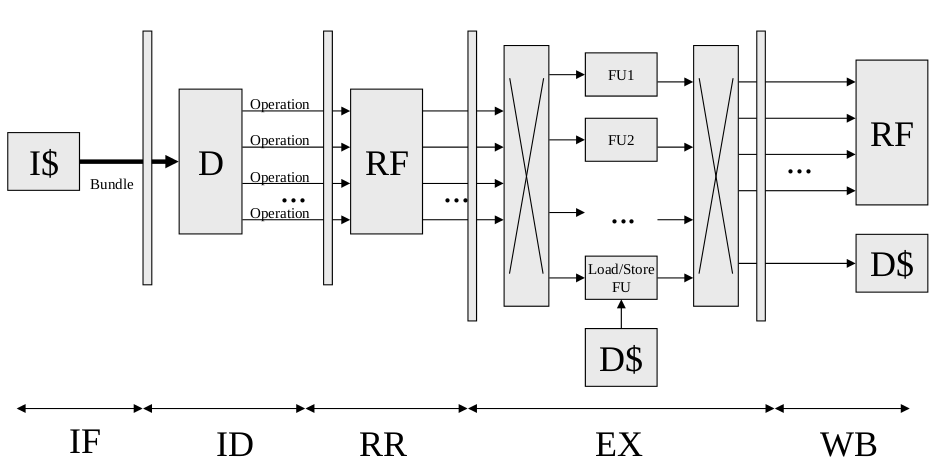
\includegraphics[scale=0.5]{img/vliwarch.png}
\caption{Architettura di una pipeline per VILW}\label{fig:vliwarch}
\end{figure}